% Appendix 5: The Occurrence of Reverse Perspective at Close Distances
%             due to the Phenomenon of "Superconstancy"
% Source pages: 260–262

\chapter{The Occurrence of Reverse Perspective at Close Distances due to
  the Phenomenon of ``Superconstancy''}

The size-constancy mechanism is sufficiently effective that over limited distances complete
constancy is frequently observed.  In the classic experiments of Holway and
Boring,\footnote{A.\,H.~Holway, E.\,G.~Boring.  Determinants of apparent visual size
  with distance variant.---\emph{Amer.\ J.\ Psychol.}, 1941, 54, pp.\,21--37.  The
  experimental results of these authors are here processed by a method different from that
  given in their paper.} an observer stationed at the intersection of two darkened corridors
was presented with illuminated discs (one in each corridor).  The first disc was at a fixed
distance ($\sim 3$~m) from the observer, who could adjust its diameter to match that of the
second disc, which was placed in the other corridor.  The second disc was placed at various
distances from the observer (from $\sim 3$ to $\sim 36$~m), its linear size being varied so
that its angular size remained constant at $1°$.  With monocular vision, complete constancy
was registered at all distances, i.e.\ the observer matched the size of the first disc to the
second essentially without error.  With binocular vision, ``superconstancy'' was noted:
the observer selected the diameter of the first disc as \emph{larger} than the second.

Fig.\,5.1 shows the summary diagram.  The abscissa gives the distance to the second disc,
the ordinate the ratio of diameters (first to second).  The following is characteristic of
the entire array of experimental points: with increasing distance to the second disc up to
about 15~m, all observers overestimated its size (unanimous ``superconstancy''), which is
seen from the fact that the experimental points lie above the dashed line corresponding to
ideal constancy; for distances 15--36~m the picture becomes more complex, and the scatter
of experimental points increases with a clear tendency towards decreasing effectiveness of
the size-constancy mechanism.

\begin{figure}[H]
    \centering
    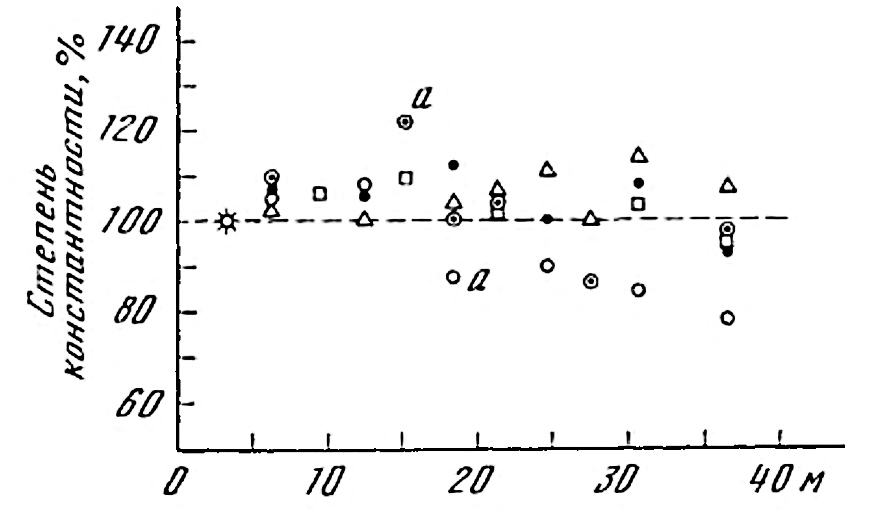
\includegraphics[width=0.65\linewidth]{figures/f5.1.png}
\end{figure}
\figblock{5.1}{Summary diagram of the Holway--Boring experiment: ratio of disc diameters
  (first/second) vs.\ distance to second disc.  Points above the dashed line correspond to
  ``superconstancy''.}

\begin{figure}[H]
    \centering
    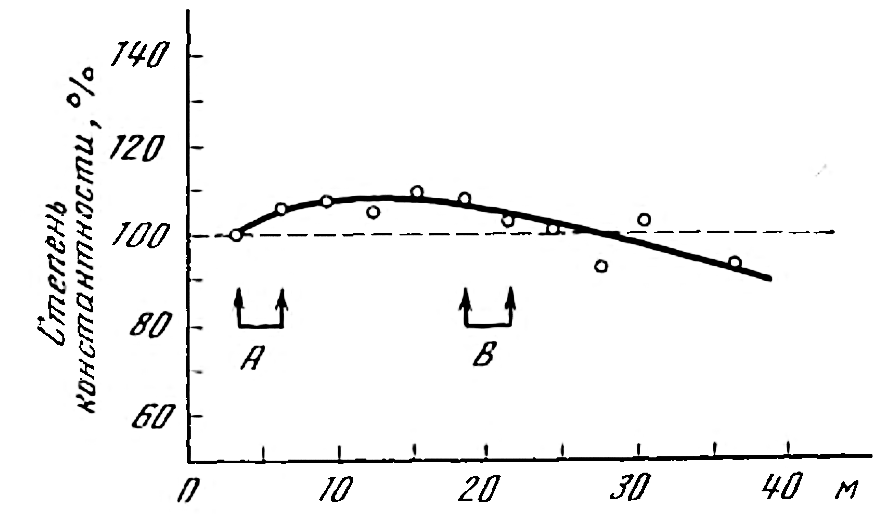
\includegraphics[width=0.65\linewidth]{figures/f5.2.png}
\end{figure}
\figblock{5.2}{Curve of mean constancy vs.\ distance, derived from Fig.\,5.1.  The maximum
  occurs at 10--15\,m.  Reverse perspective can occur only to the left of the maximum (up
  to $\sim$10\,m); to its right, widths progressively decrease.}

In those cases where the phenomenon of ``superconstancy'' was not observed in other
experiments (since the numerical values in such experiments depend strongly on experimental
methodology), the increase of constancy in the transition from monocular to binocular
vision was nonetheless firmly established.  Thus in the experiments of A.\,A.~Smirnov and
M.\,N.~Volokitina,\footnote{A.\,A.~Smirnov, M.\,N.~Volokitina.  Dependence of the
  constancy of the perceived size of objects on their mutual separation at various observation
  distances.---In: \emph{Visual Sensations and Perceptions}, Moscow--Leningrad, 1935.}
the increase of constancy in the transition from monocular to binocular vision averages
5--10\%, i.e.\ it is of the same order as in the Holway--Boring experiments.

\srcpage{261}

One should not think that the location of experimental points above the dashed line in
Fig.\,5.1 itself testifies to the emergence of the reverse-perspective effect.  To clarify
this, refer to Fig.\,5.2, which shows the curve of the arithmetic mean constancy obtained
by processing the experimental points of Fig.\,5.1.

The graph in Fig.\,5.2 shows a maximum degree of constancy in the distance range 10--15~m.
The reverse-perspective effect can be observed only to the left of the maximum, i.e.\ at
distances up to about 10~m, since the essence of reverse perspective is the increase of
lateral size with distance, while to the right of the maximum a progressive decrease in this
size will occur.  Indeed, a rectangular object of depth 3~m whose front face is 3~m from
the observer will have a visible size of its far edge 5\% larger than the front (region~$A$
in Fig.\,5.2), while if shifted to a distance of $\sim 18$~m it will be characterised by a
decrease of the visible size of the far edge relative to the front by 2\% (region~$B$ in
Fig.\,5.2).  Thus it is not the very fact of superconstancy but the \emph{increase} of the
degree of constancy with distance that is decisive for the emergence of the reverse-perspective
effect.  If one takes as a basis the data from the Holway--Boring experiments, the
``natural'' reverse-perspective effect associated with the binocularity of human vision
should be observed at distances up to 10~m.

Using the initial, steepest part of the curve shown in Fig.\,5.2, corresponding to distances
3--6~m, one can estimate the degree of expression of the reverse-perspective perception.
If these data are used to determine the visual appearance of a rectangle having an aspect
ratio of 1:3 with its long side oriented away from the observer, the calculations give the
degree of divergence of the parallel lines in visual perception as of the order of $2°$, i.e.\
the effect described here can lead to only a very weak reverse perspective.

\srcpage{262}

In Appendices~2 and~3 a mathematical description of a simplified perceptual perspective
system was given, in which the function $P_1$ was determined from conditions corresponding
to monocular vision.  To determine the function $P_1$ from the laws of binocular vision,
it suffices to modify condition~(2.3) as follows:
\begin{equation}
  \frac{dP_1}{dl}(0) = 1 + \alpha,  \tag{5.1}
\end{equation}
where $\alpha > 0$, and the quantity~$\alpha$ should be determined from experiment (e.g.\
from the experiment described in the present Appendix).
